% Generated by scripts/supp_tex.py from scripts/supp/e_budget.py.
% Do not edit: edit the module, which also builds the PDF version.

\section{The operating window}
\label{supp:e_budget}

A budget D is the peak-signal-to-noise ratio the decode is allowed to give up, and an allocation is admissible if the loss it incurs stays at or below it. Between a floor, below which no allocation is admissible, and a saturation point, above which every allocation has reached the same ceiling, lies the window of budgets in which the decoder has anything to trade. Section C derives the two ends and Section D tabulates them. This section is about the window itself.

It covers how the two ends are measured and how far the measurements agree, what has to be stated with every decibel before any of it means anything, the sweep across the whole window, and how much of the rescaling that collapses the five rates onto one curve survives a change of sweep, of convention or of checkpoint.

\subsection{Floor, saturation point and ceiling}

The floor D\_min is the loss of a tiled decode with every tile at full depth. No early exiting has happened, so it is the tiling penalty alone: the border of every tile has been convolved against padding rather than against its neighbour. The saturation point D\_sat is the loss when every tile takes exit j, the shallowest the split depth allows. Neither is a quantity to search for. Each is one forward pass per rate with the exit map held constant, which is what makes the rescaling in Section A.4 cheap enough to be worth doing in deployment.

Between them the saving is fixed by the ladder rather than by the budget. With c\_k the cost of exit k in units of one released full-frame decode, j the split depth and K the number of exits, the ceiling is closed form under either compute denominator:

\begin{equation}
S_{\mathrm{max}}^{\mathrm{rel}} = 100\,(1 - c_j), \;\; S_{\mathrm{max}}^{\mathrm{self}} = 100\,(1 - c_j/c_{K-1}),
\end{equation}

With c\_j = 0.6088, recorded in results/saturation\_RECIPE512\_ctc53.json, and c\_(K$-$1) = 1.0095, recorded as deepest\_exit\_cost in results/router\_RECIPE512\_b01.json, the first reads \CeilingModelled\% and the second 39.7\%. The deepest exit costs more than one released decode because it carries the seam repair, which the released decoder does not run, and that difference is the whole of the gap between the two ceilings.

Section D tabulates both ends at all nine measured rates, and that table is not repeated here. The one property of it this section needs is that a budget in decibels means something different at each rate: both ends widen as the rate falls, the band widens faster than the floor rises, and the 0.1 dB budget that sits \BandUseLow\% of the way up the band at q0 sits \BandUseHigh\% of the way up at q63. The rescaling of Section A.4 turns out to need that position rather than the decibel figure.

A budget below the floor admits no allocation at all, which is a different failure from a budget falling in a gap of the Lagrangian hull, where the sweep returns the nearest reachable point and Everett's argument still makes it optimal for the compute it consumes [26, 27]. Below the floor the feasible set is empty and there is nothing to return. Three cells of the grid in Section A.3 are in that state and are recorded as such rather than dropped: at a 0.05 dB budget the three highest rates, q32, q48 and q63, have floors of 0.053, 0.060 and 0.066 dB.

Three estimates of the floor are in play and they are not interchangeable. Table 1 gives all three, because the rescaling below divides by the distance between the floor and the saturation point, and near the floor that is a small difference divided by a small difference.

\begin{table}[t]
\centering
\resizebox{\columnwidth}{!}{%
\begin{tabular}{lrrr}
\toprule
source & what it measures & q0 & q63 \\
\midrule
the saturation file & a deployed decode with every tile at full depth, over \NumSeq frames & \FloorLow & \FloorHigh \\
the dense grid & the same quantity, over 106 frames & 0.033 & 0.066 \\
the second sweep & the per-tile table at a zero multiplier, where a tile takes its own lowest-error exit & - & 0.066 \\
\bottomrule
\end{tabular}}
\caption{\textbf{Three measurements of the floor, in decibels.} The first two differ by three to six thousandths of a decibel because they are the same quantity over a different number of frames. The third is a different quantity: a tile whose shallower exit happens to have the lower error takes it, so the table's floor sits below the deployed one. Everything downstream of here takes both ends of the window from the first row, so that the floor and the saturation point are on one measurement.}
\end{table}

{\small The three rows are results/saturation\_RECIPE512\_ctc53.json, results/signalled\_RECIPE512\_grid.json and results/supp\_paper\_curve\_PAPER.json, all on the pinned checkpoint and all with decibels averaged per frame. The third records a floor only where it found the 0.05 dB budget unreachable, which is why q0 is empty.}

\begin{figure}[t]
\centering
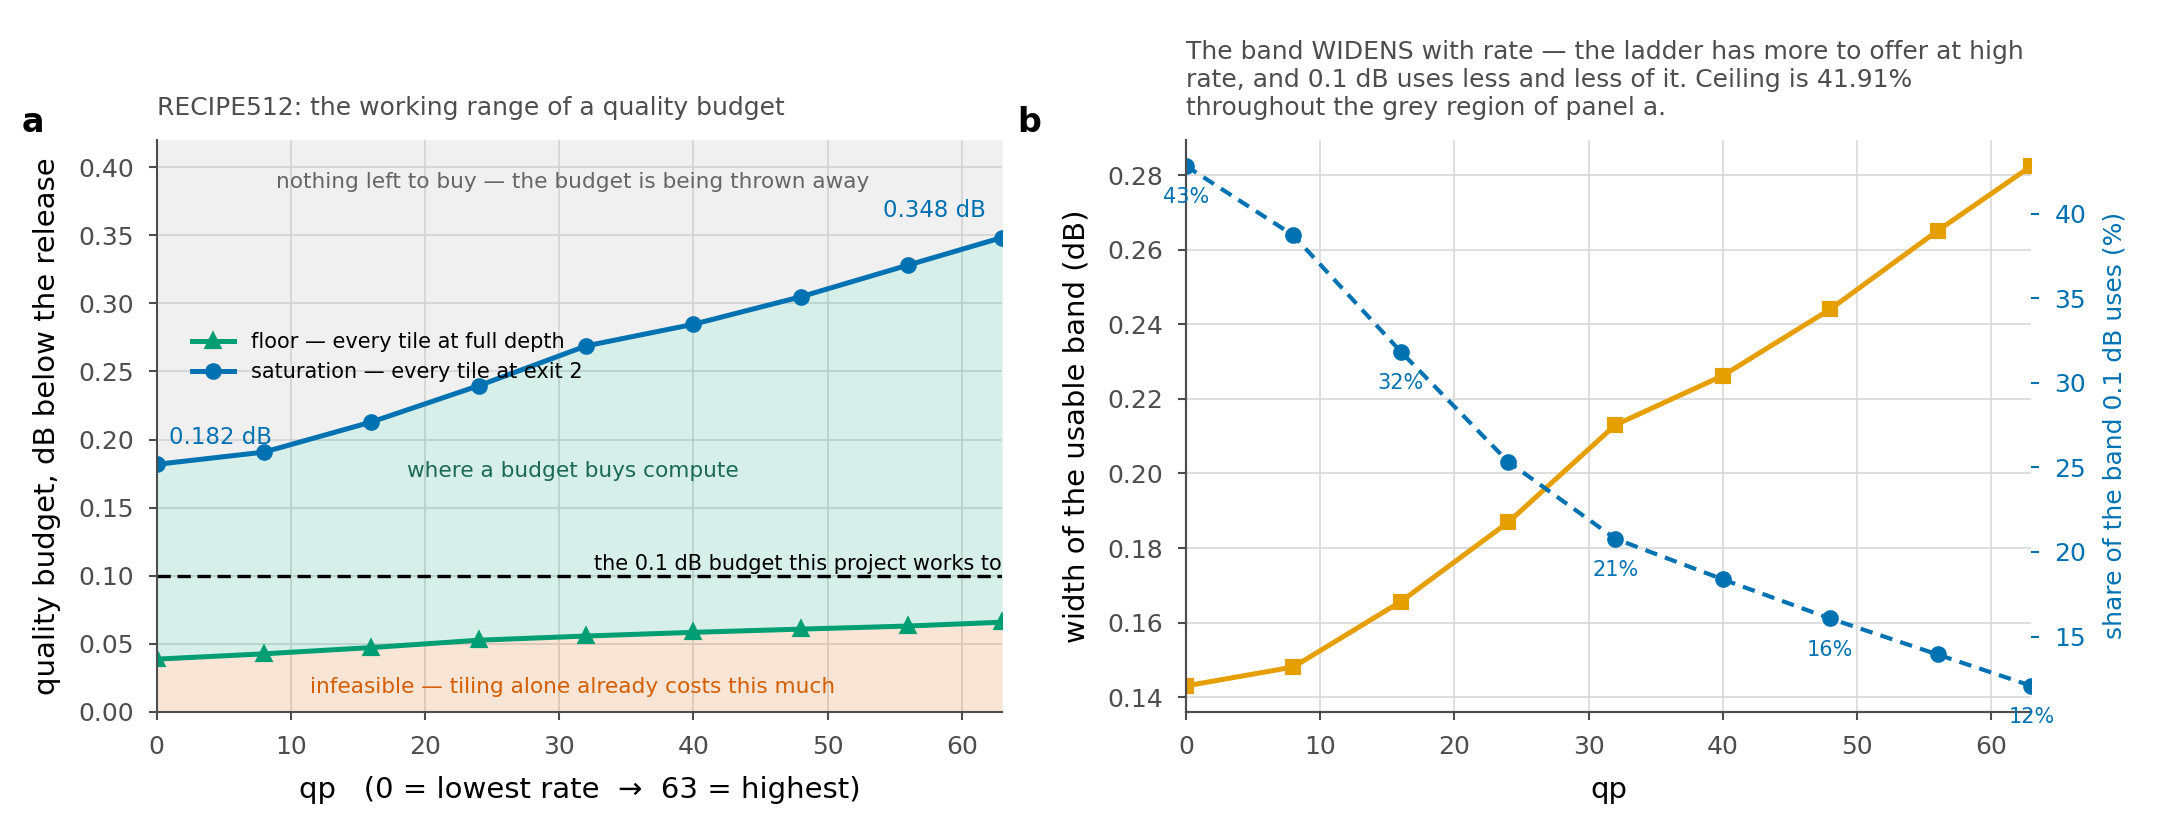
\includegraphics[width=\columnwidth]{figures/saturation_RECIPE512.png}
\caption{\textbf{Three regions, and only the middle one is a design choice.} Below the floor no allocation meets the budget; above saturation every tile already takes the cheapest exit and a looser budget buys nothing. The 0.1 dB budget uses \BandUseLow\% of the band at the lowest rate and \BandUseHigh\% at the highest, which is why the same budget behaves so differently at the two ends of the rate range.}
\end{figure}

\begin{figure}[t]
\centering
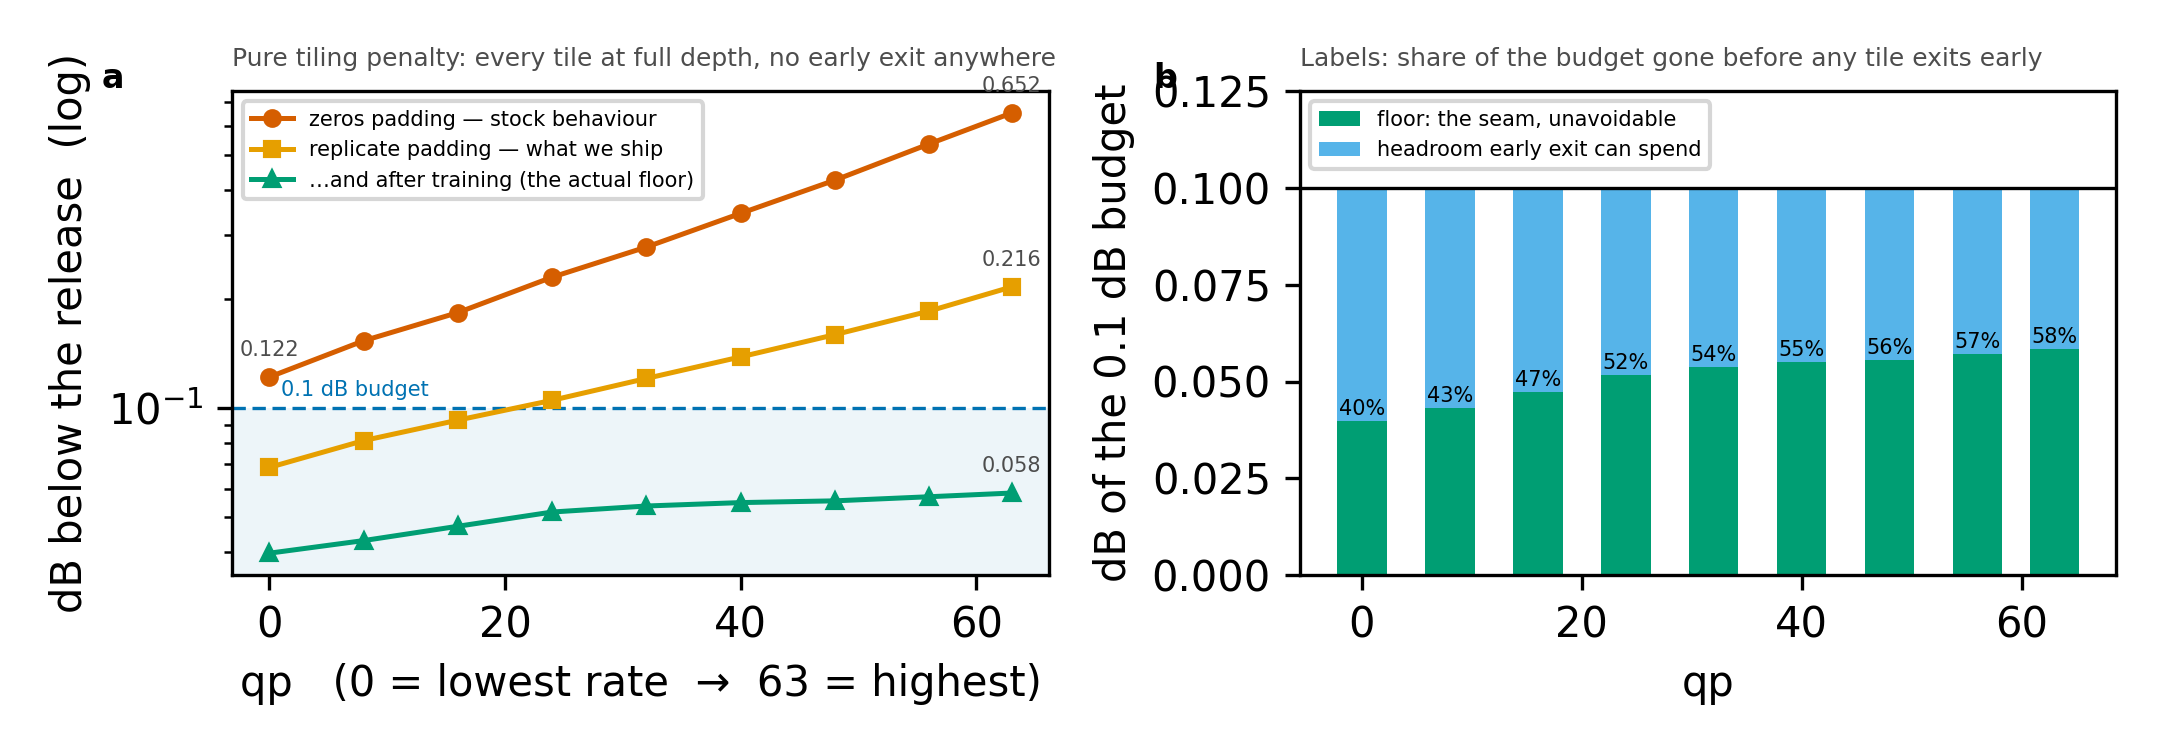
\includegraphics[width=\columnwidth]{figures/seam_vs_qp.png}
\caption{\textbf{The tiling penalty across the whole rate range}, every tile at full depth, so this is the floor and nothing else. \textbf{a}, the steps that reduce it, of which the two that matter cost no arithmetic; the largest single factor is training the ladder with the seam present. \textbf{b}, the floor as a share of the 0.1 dB budget: it is charged \emph{inside} the budget and consumes a growing part of it as the rate rises, which is one of the two reasons the saving falls with rate.}
\end{figure}

\subsection{Three conventions, and the conversions between them}

Three separate choices have to be pinned before a figure in this section means anything, and the project makes all three in two ways in different files. The loss can be measured against the released decoder's full-frame decode of the same latent, which puts the cost of cutting the frame into tiles inside the budget, or against this model's own deepest exit decoded tile by tile, which cancels it. Decibels can be averaged per frame and then over frames, which is what the released codec's own evaluation does, or pooled into one mean squared error first. And the saving can be divided by the released decode or by our own deepest exit. Two of the three conversions are exact:

\begin{equation}
D^{\mathrm{rel}} = D^{\mathrm{self}} + D_{\mathrm{min}}, \;\;\; S^{\mathrm{rel}} = 100 - c_{K-1}\,(100 - S^{\mathrm{self}}).
\end{equation}

\begin{table}[t]
\centering
\resizebox{\columnwidth}{!}{%
\begin{tabular}{lrr}
\toprule
choice & the two options & what separates them \\
\midrule
loss measured against & the released full-frame decode, or our own tiled deepest exit & the floor: \FloorLow dB at q0, \FloorHigh dB at q63 \\
decibels averaged & per frame and then over frames, or pooled over every tile first & measured, not closed form: a pooled 0.1 dB is 0.117 dB per frame at q0 and 0.122 at q63 \\
saving divided by & the released decode, or our deepest exit at 1.0095 of it & a self-referenced 30\% is 29.33\% release-referenced, and a self-referenced 0\% is $-$0.95\% \\
\bottomrule
\end{tabular}}
\caption{\textbf{What has to be stated with every decibel and every saving in this section.} Take from it that a number quoted without its convention is uncertain by about a third of a 0.1 dB budget on the quality axis and by about two thirds of a point on the compute axis. The first and third rows convert exactly, by the identity above; the second does not, because a mean of logarithms is not the logarithm of a mean.}
\end{table}

{\small The floor is results/saturation\_RECIPE512\_ctc53.json; the two averaging figures are the 0.1 dB operating points of results/supp\_paper\_curve\_PAPER.json, which bisects on the pooled decibel and records the per-frame decibel of the same allocation beside it; the deepest-exit cost is deepest\_exit\_cost in results/router\_RECIPE512\_b01.json. The averaging convention itself is defined in Section A.}

\subsection{The grid}

Table 3 is the sweep the main paper quotes: nine budgets across five rates, measured against the released decoder on both axes, with decibels averaged per frame, two frames from each of the \NumSeq test sequences. Allocation is by the exact per-tile losses, so every entry is an upper bound on what a decoder-side router can reach.

\begin{table}[t]
\centering
\resizebox{\columnwidth}{!}{%
\begin{tabular}{lrrrrr}
\toprule
budget dB & q0 & q16 & q32 & q48 & q63 \\
\midrule
0.050 & 16.4 & 9.3 & none & none & none \\
0.075 & 24.3 & 19.7 & 14.6 & 11.1 & 7.6 \\
0.100 & 29.8 & 25.5 & 20.7 & 18.2 & 15.6 \\
0.150 & 36.6 & 33.0 & 28.6 & 26.5 & 24.1 \\
0.200 & 39.1 & 37.8 & 33.7 & 31.6 & 29.6 \\
0.250 & 39.1 & 39.1 & 37.4 & 35.2 & 33.0 \\
0.300 & 39.1 & 39.1 & 39.1 & 37.9 & 35.8 \\
0.400 & 39.1 & 39.1 & 39.1 & 39.1 & 39.1 \\
0.500 & 39.1 & 39.1 & 39.1 & 39.1 & 39.1 \\
\bottomrule
\end{tabular}}
\caption{\textbf{Compute saved against budget, release-referenced.} \emph{none} marks a budget below that rate's floor, where no allocation is admissible. Reading down a column, the return on a looser budget falls away long before the ceiling is reached. Reading across a row, the rate dependence is largest at the tightest budget and vanishes once every rate has saturated. Cells are the cost model against the release, the convention the rest of this supplement compares in; hook-counted, the 0.1 dB row reads 29.1\% at q0 and 15.2\% at q63, which reproduces the headline of the main paper, \MainLowRate\% and \MainHighRate\%, to within a tenth of a point on a different frame count.}
\end{table}

{\small results/signalled\_RECIPE512\_grid.json, pinned checkpoint, two frames per sequence, budget bisected on the delivered per-frame decibel of a real decode of the mixed map. The headline file results/signalled\_RECIPE512\_ctc53.json uses one frame per sequence and reports \MainLowRate\% and \MainHighRate\% at the same budget.}

A second sweep of the same checkpoint prices the same window differently, and Section D prints its operating points in full. It bisects on the pooled decibel rather than the per-frame one and reads \NumSeq sequences at one frame each rather than two, and at a nominal 0.1 dB it saves several points more at every rate than the grid above. The conversions of Section A.2 account for part of that and not for all of it, which is the first sign of what Section A.5 measures. Its own saturation points are the useful thing here: the budget at which a rate runs out of allocation is 0.20 dB at q0, 0.25 dB at q16, 0.30 dB at q32, 0.50 dB at q48, 0.50 dB at q63. The three budgets the paper reports are therefore not three points on one curve. At 0.1 dB every rate still has an allocation to make, at 0.3 dB only q48 and q63 do, and at 0.5 dB none does.

{\small results/supp\_paper\_curve\_PAPER.json, pinned checkpoint, \NumSeq sequences at one frame each, 35 operating points at seven budgets. A saturated point is flagged in the file rather than inferred here, and carries no exit histogram, because the allocation has stopped changing.}

Budgets in [\SatLow, \SatWindowHi) dB saturate the lowest rate and no other, a window \SatWindowMb thousandths of a decibel wide. Above \SatHigh dB every rate has saturated, so the binding constraint is the ladder rather than the budget. Both figures are read off the nine-rate table in Section D rather than off either sweep.

\subsection{Rescaling onto the band}

With both ends of the window measured, a budget can be quoted as a position in the window rather than as a decibel figure. Write

\begin{equation}
u = \frac{D - D_{\mathrm{min}}}{D_{\mathrm{sat}} - D_{\mathrm{min}}},
\end{equation}

so that u = 0 is the floor and u = 1 the saturation point. At a matched decibel the five rates are \BandRawSpread points apart in saving. At a matched u they are \BandSpreadMean points apart on average and \BandSpreadMax at worst, so the window accounts for most of the rate dependence of the trade-off and a couple of points are left over.

\begin{table}[t]
\centering
\resizebox{\columnwidth}{!}{%
\begin{tabular}{lrrrrrr}
\toprule
u & q0 & q16 & q32 & q48 & q63 & spread \\
\midrule
0.1 & 16.5 & 14.6 & 15.1 & 15.2 & 16.3 & 1.91 \\
0.2 & 21.0 & 20.9 & 20.7 & 20.9 & 21.8 & 1.13 \\
0.3 & 25.2 & 24.9 & 24.3 & 25.5 & 26.2 & 1.91 \\
0.4 & 28.3 & 27.7 & 27.9 & 28.6 & 29.7 & 1.96 \\
0.5 & 30.8 & 30.4 & 30.4 & 31.4 & 31.9 & 1.54 \\
0.6 & 32.8 & 33.0 & 32.8 & 33.4 & 33.9 & 1.13 \\
0.7 & 34.7 & 34.7 & 34.7 & 35.3 & 35.7 & 1.00 \\
\bottomrule
\end{tabular}}
\caption{\textbf{The five rates at matched positions in their own windows.} Read across a row: five rates whose raw savings at a matched decibel differ by \BandRawSpread points agree here to about a point and a half. The spread is largest at the bottom of the window, where the floor subtraction is a large fraction of a small number and the two files disagree about the floor by a few thousandths of a decibel.}
\end{table}

{\small Computed in the build from results/signalled\_RECIPE512\_grid.json and results/saturation\_RECIPE512\_ctc53.json by the rescaling in scripts/tradeoff\_figure.py, linearly interpolated between measured points. Every rate has measured points spanning u = 0.10 to 0.70, so no entry is an extrapolation. Mean spread over these seven positions 1.51 points, worst 1.96, against the \BandSpreadMean and \BandSpreadMax recorded in results/band\_collapse.json, which interpolates on a wider grid and holds the last measured value beyond each rate's last point.}

The collapsed curve is then described by one free number. With C the architectural ceiling, which is not fitted,

\begin{equation}
S(u) \approx C\,u^{\beta},
\end{equation}

and fitting ln(S/C) against ln u by least squares through the origin gives \BandExp on the pinned checkpoint, with R$^2$ = \BandRTwo and a worst residual of \BandFitErr points. The same procedure on the second training run gives \BandExpB with R$^2$ = \BandRTwoB, which is the replication Figure 3 draws and Section A.5 takes apart.

\begin{figure}[t]
\centering

\includegraphics[width=\columnwidth]{figures/budget_band_BEST.png}
\caption{\textbf{The collapse on the second training run.} \textbf{a}, saving against budget, one line per rate, with each rate's floor and saturation point ticked. \textbf{b}, the same with the budget axis rescaled onto each rate's own window; dashed is the one-parameter power law. The main paper shows this pair for the pinned checkpoint.}
\end{figure}

{\small docs/figures/budget\_band\_BEST.png, drawn by scripts/tradeoff\_figure.py from results/signalled\_BEST\_grid.json and results/saturation\_BEST\_ctc53.json, both on runs/BEST/ckpt\_eval.pth.tar rather than on the pinned checkpoint.}

\begin{figure}[t]
\centering
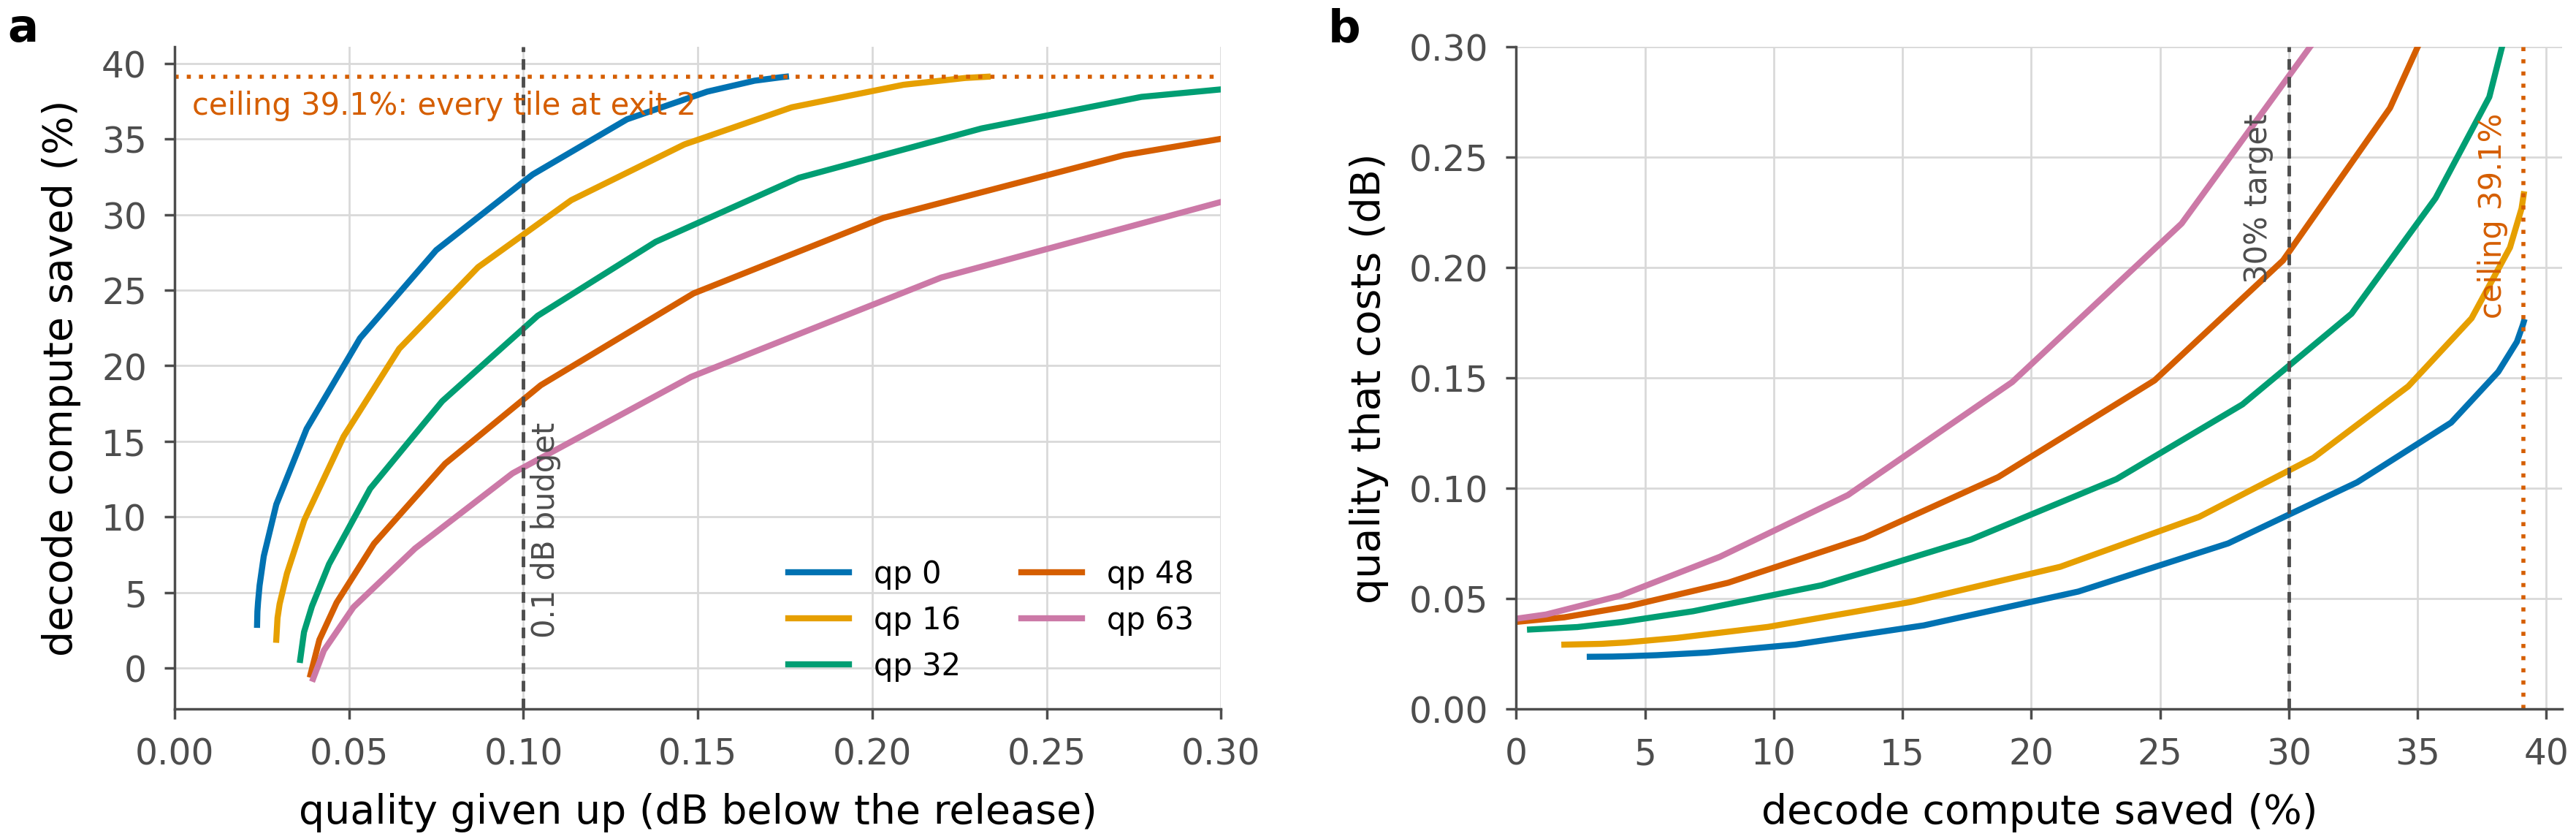
\includegraphics[width=\columnwidth]{figures/tradeoff.png}
\caption{\textbf{The trade-off, whole.} \textbf{a}, what a budget buys, per rate; the ceiling is \Ceiling\% and q0 reaches it at \SatLow dB. \textbf{b}, the same relation inverted, so it reads as what a saving target costs in quality. The budgets the main paper reports are three points on this curve, and the flat right-hand end of each trace is that rate sitting on the ceiling.}
\end{figure}

\subsection{How weak the replication is}

The main paper says the collapse replicates and the exponent does not. Two checkpoints is a thin basis for either half of that sentence, and Table 5 is meant to show how thin. Each row refits the same one-parameter law after changing exactly one thing, over the window of positions where every sweep has points.

\begin{table}[t]
\centering
\resizebox{\columnwidth}{!}{%
\begin{tabular}{lrrr}
\toprule
what is changed & $\beta$ before & $\beta$ after & $\Delta$ \\
\midrule
the checkpoint, pinned to BEST, each with its own ceiling & 0.360 & 0.310 & -0.050 \\
the sweep, 106 frames to \NumSeq, one checkpoint & 0.360 & 0.261 & -0.098 \\
the budget axis, per-frame decibels to pooled, one sweep & 0.272 & 0.180 & -0.093 \\
the assumed ceiling C, \CeilingModelled to 41.91 & 0.360 & 0.421 & 0.061 \\
the floor, the saturation file to the grid's own & 0.360 & 0.369 & 0.010 \\
the rate, fitted one at a time, q63 against q32 & 0.321 & 0.385 & 0.064 \\
the fit form, 1/b from the inverse fit, per rate & 0.326 & 0.459 & 0.133 \\
\bottomrule
\end{tabular}}
\caption{\textbf{What moves the exponent.} Take from it that the exponent describes a sweep rather than a decoder. Every row except the floor moves it by as much as changing the checkpoint does, re-sweeping the same checkpoint moves it twice as far, and reading the budget axis in the other averaging convention moves it almost as far again. The comparison the main paper draws between \BandExp and \BandExpB is inside the noise of every other choice on this list.}
\end{table}

{\small Computed in the build. Rows 4, 5 and 6, and the before column of rows 1 and 2, refit results/signalled\_RECIPE512\_grid.json against results/saturation\_RECIPE512\_ctc53.json; the after column of row 1 uses results/signalled\_BEST\_grid.json and results/saturation\_BEST\_ctc53.json on runs/BEST/ckpt\_eval.pth.tar, whose ceiling is its own; the after column of row 2 uses the operating points of results/supp\_paper\_curve\_PAPER.json and row 3 uses its raw sweep; row 7 is results/frontier\_law.json, fitted to results/curve\_BEST.json on the same second run over 40 sequences. Every fit is over u in [0.15, 0.85] and through the origin in log space, on 16 to 22 points. R$^2$ stays between 0.911 and 0.980 across the rows, so no row is a bad fit to its own data.}

\begin{figure}[t]
\centering
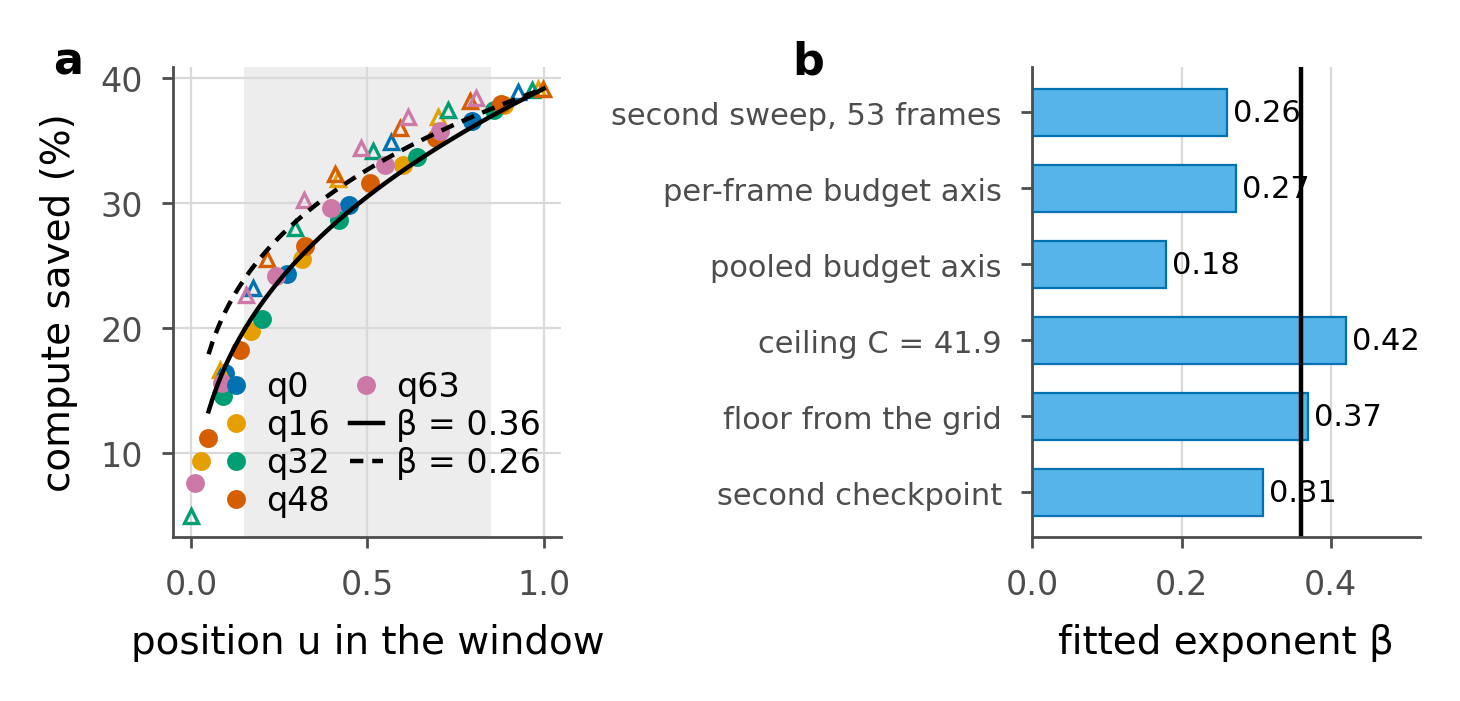
\includegraphics[width=\columnwidth]{figures/band_sensitivity_PAPER.png}
\caption{\textbf{The collapse, and what the exponent is sensitive to.} \textbf{a}, the rescaled points from two sweeps of the pinned checkpoint, filled circles for the 106-frame grid and open triangles for the \NumSeq-frame frontier, with the power law fitted to each over the shaded window. The two sweeps of one checkpoint do not lie on one curve. \textbf{b}, the exponent under one change at a time, with the vertical line at the exponent of the first row of Table 5. The change of checkpoint, which the main paper reads as a finding, is the smallest of the six.}
\end{figure}

{\small docs/figures/band\_sensitivity\_PAPER.png, drawn by scripts/supp\_fig\_band\_sensitivity.py, which imports the fit from this section's module so that the figure and the table cannot disagree. Sources as for the table above.}

The floor is the one input the exponent is insensitive to over this window, and only over this window. Refitting over the whole range instead, where the points below u = 0.15 sit, moves it from 0.379 to 0.417 when the floor is taken from the grid rather than from the saturation file. A rescaling is only as good as the two numbers it divides by, and near the floor it is dividing a small difference by a small difference.

Both fits are re-run in this build from the files they name, so the exponent quoted here is the exponent those inputs now support: results/band\_collapse\_BEST.json reproduces at 0.3253 with R$^2$ = 0.9843 against the 0.2827 and 0.9068 it records, and the two digits the paper quotes, \BandExp and \BandRTwo, are unchanged by the exercise.

\subsection{Which ladder a budget wants}

Once a budget saturates a ladder, the only way to spend more quality is an exit that does not exist, so the ladder itself is a choice made at the operating point rather than a hyperparameter tuned once. Four ladders have been run far enough to compare, and the two orderings cross between 0.1 and 0.3 dB.

\begin{table}[t]
\centering
\resizebox{\columnwidth}{!}{\begin{tabular}{llrrrrrr}
\toprule
Config & Ep. & $q0$ & $q16$ & $q32$ & $q48$ & $q63$ & mean \\
\midrule
RECIPE512 & 0 & 33.2 & 29.5 & 24.4 & 21.4 & 18.8 & 25.4 \\
BEST & 1 & 34.6 & 28.9 & 24.0 & 21.7 & 18.8 & \textbf{25.6} \\
\bottomrule
\end{tabular}
}
\caption{\textbf{Ladder settings}, mean saving over the five rates, on each run's own latest checkpoint. Ceilings are 100(1 $-$ c\_j) for that ladder, corrected by the offset the hook count shows. The asterisk marks a setting where some rate did not reach the budget, so the mean is over the rest; the dagger marks a saving taken from the arithmetic model rather than counted off the decode, which reads 0.4 to 0.8 points optimistic. Only RECIPE512 has been re-measured with hooks at every budget, and it is the only run the main paper reports.}
\end{table}

{\small The four signalled\_*.json curve files named in scripts/make\_paper\_tables.py, generated into paper/tables/runs.tex. The four runs are at different epochs, so no row here separates a ladder from the run that trained it; section H measures how far two runs of one recipe land apart.}

At 0.1 dB the coarse ladder wins and the fine one (K = 12, j = 4) cannot reach the budget at the highest rate at all. Splitting later puts twice as many blocks in the per-tile section, and the seam penalty grows with that count, so a finer ladder raises the floor it has to clear before it can spend anything. At 0.5 dB the fine ladder wins, \FineHalfDb\% against \CoarseHalfDb\%, because the coarse one has been pinned at its ceiling since 0.3 dB and has nothing left to spend. The band of E.1 says which side of that crossover a given budget sits on, which is the practical use of measuring the two ends.

\subsection{What the window claims, and what it does not}

\begin{itemize}\itemsep1pt
\item The floor and the saturation point are measured, cheap and unambiguous. Each is one forward pass per rate, and the ceiling between them is closed form in the per-exit costs.
\item The collapse is the claim. Rescaling a budget onto its own window takes the spread across rates from \BandRawSpread points to under two at matched positions, on both checkpoints.
\item The exponent is an empirical fit and a description of one sweep, not a law. It moves further when the same checkpoint is swept again, or when the budget axis is read in the other averaging convention, than it moves between the two training runs the main paper compares.
\item Everything here is the oracle allocation, obtained with the per-tile losses known. It bounds any router and says nothing about how much of the window a decoder-side predictor reaches, which is what Section F measures.
\end{itemize}

